\chapter{Reproducible finite experiments and interactive geometry}

\section{What the computations verify}

The computational companion has two independent implementations of the
principal finite examples: Python for the paper's exact checks and figures,
and JavaScript for the interactive page. Both are deliberately small. Their
purpose is to make definitions inspectable, expose exceptional cases, and
check consistency between formulas and displays. Neither is an implementation
of production cryptography or a simulator of continuum Yang--Mills theory.

The Python script \path{code/verify_examples.py} uses only the standard
library.

It writes \path{verification/examples.json}, including a SHA-256
hash of the script, exact finite counts, and numerical residuals. The figure
script additionally uses NumPy and Matplotlib. The browser experiments are
buildless and use no remote JavaScript dependency. A separate Node script
\path{site/verify-math.cjs} checks the shared mathematical functions used
by the interface. The environment and invocation commands are recorded in
the project README.

It is important to distinguish three kinds of evidence. A symbolic proof
establishes an identity for all objects under its assumptions. Exhaustive
finite enumeration establishes a property of the enumerated finite
structure. A floating-point residual checks a sampled numerical
implementation up to a tolerance. The companion labels these categories
explicitly. For example, checking $BA=0$ to $10^{-12}$ at sample points on a
projected cone is not a proof of exactness, and a table of 19 elliptic-curve
points is not a proof of the group law for every elliptic curve.

\section{The 19-element elliptic-curve example}

The curve
\[
 E:\quad y^2=x^3+2x+2\quad\text{over }\F_{17}
\]
has 18 affine points and one point $O$ at infinity. The enumeration checks
every pair $(x,y)\in\F_{17}^2$ directly. It also checks that
$P=(5,1)$ has order 19 and generates the entire set. The affine formulas
treat the identity, inverse pairs and tangent cases separately. This is
essential: blindly inverting a zero denominator would invalidate the
implementation.

\begin{center}
\begin{tabular}{rrrr}
\toprule
$k$ & $kP$ & $k$ & $kP$\\
\midrule
0 & $O$ & 10 & $(7,11)$\\
1 & $(5,1)$ & 11 & $(13,10)$\\
2 & $(6,3)$ & 12 & $(0,11)$\\
3 & $(10,6)$ & 13 & $(16,4)$\\
4 & $(3,1)$ & 14 & $(9,1)$\\
5 & $(9,16)$ & 15 & $(3,16)$\\
6 & $(16,13)$ & 16 & $(10,11)$\\
7 & $(0,6)$ & 17 & $(6,14)$\\
8 & $(13,7)$ & 18 & $(5,16)$\\
9 & $(7,6)$ & 19 & $O$\\
\bottomrule
\end{tabular}
\end{center}

The exact test enumerates all $19^3=6,859$ triples and checks associativity
with modular integer arithmetic. It checks closure and commutativity on all
pairs. Finally, for each of the 19 choices of $d$, it enumerates the kernel of
$(a,b)\mapsto aP+b(dP)$ and compares it to
$\{(-dt,t):t\in\Z/19\Z\}$. This last comparison connects the concrete curve
display to the hidden-subgroup theorem in the text.

\begin{figure}[htbp]
\centering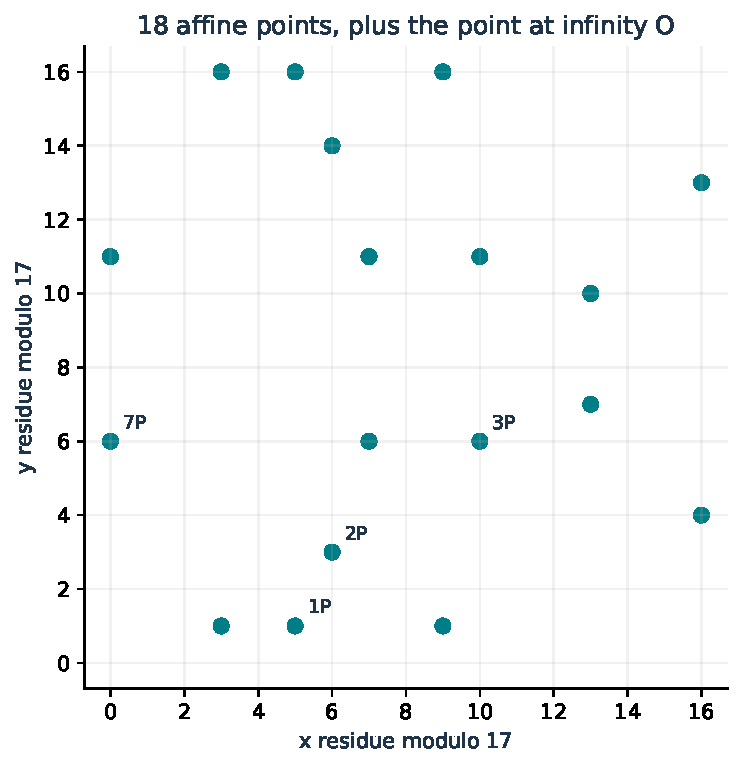
\includegraphics[width=.80\textwidth]{figures/ecc17.pdf}
\caption{The finite-field curve is a discrete set of residues. The straight
layout of the residue grid is a display convention; it is not the real
plane cubic, and Euclidean distances between the plotted dots have no role
in its group law. The point $O$ is handled separately.}
\end{figure}

The browser lets the reader select a scalar and see its corresponding point.
The small modulus makes every operation inspectable. It also makes this
example unsuitable as a security parameter: exhaustive enumeration is
intentional. The page does not accept real keys or provide an attack service.

\section{The Fourier annihilator experiment}

For the group $(\Z/7\Z)^2$ and $d=3$, the exact Fourier support is
\[
 (0,0),(1,3),(2,6),(3,2),(4,5),(5,1),(6,4).
\]
Each outcome has probability $1/7$. Every other grid point has probability
zero. The exact proof is the geometric-sum identity in the cryptography
chapter. The Python computation evaluates the complex exponential sum
numerically and compares its squared modulus with that exact probability
table. The discrepancy is recorded rather than rounded into a claim of
exact floating-point equality.

\begin{figure}[htbp]
\centering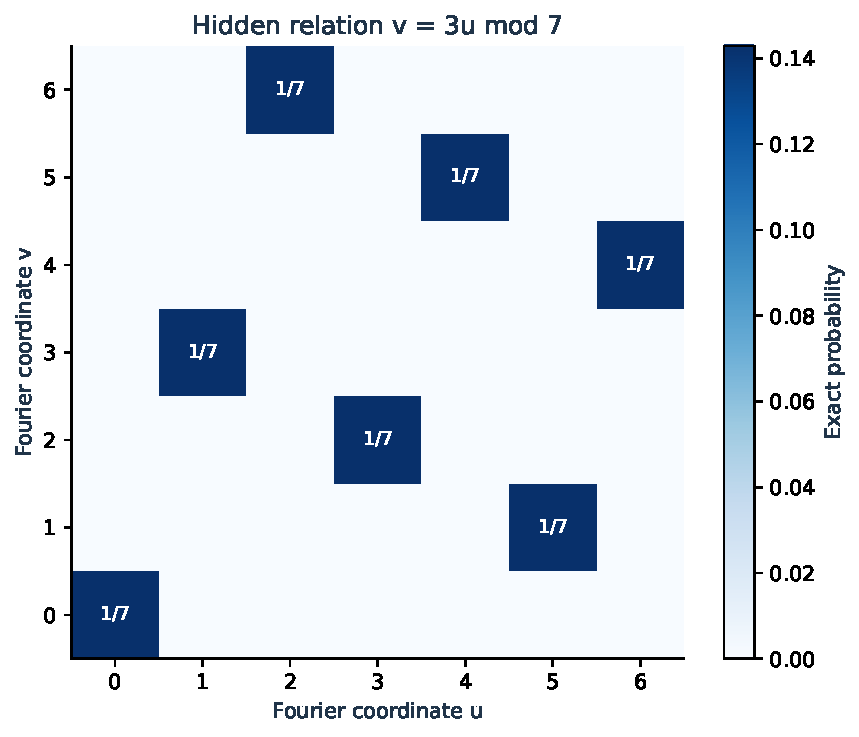
\includegraphics[width=.75\textwidth]{figures/fourier7.pdf}
\caption{Fourier mass lies on the annihilator $v=3u\pmod7$. The color bar
measures probability, not amplitude. Six of the seven possible outcomes
have nonzero $u$ and therefore recover $d$ by the stated modular inverse.}
\end{figure}

The interactive version varies the hidden slope $d$. The seven supported
points change accordingly, while the normalization remains one. This is a
finite mathematical simulation of the distribution. It does not simulate
the physical implementation of a quantum Fourier transform, and the page's
knowledge of $d$ is part of the demonstration setup. A real algorithm must
obtain its information from the oracle evaluations described in the proof.

\section{A genuine four-coordinate variety}

The variety of complexes of dimension vector $(1,2,1)$ has coordinates
\[
 A=\begin{pmatrix}x_1\\x_2\end{pmatrix},\qquad
 B=\begin{pmatrix}y_1&y_2\end{pmatrix},\qquad
 BA=x_1y_1+x_2y_2=0.
\]
The browser displays the real locus in $\R^4$. It does not identify this
four-real-dimensional ambient space with the complex variety's real
eight-dimensional ambient space. The real cone has dimension three away
from its vertex. Its unit-sphere link is two-dimensional.

Set
\[
 u=2^{-1/2}(\cos\alpha,\sin\alpha),\qquad
 v=2^{-1/2}(\cos\beta,\sin\beta),\qquad
 x=(u+v)/\sqrt2,\quad y=(u-v)/\sqrt2.
\]
Then
\[
 x\cdot y=\tfrac12(\|u\|^2-\|v\|^2)=0,
 \qquad \|x\|^2+\|y\|^2=\|u\|^2+\|v\|^2=1.
\]
The coordinate transformation is orthogonal and invertible. Its inverse
sends every point of the unit link to two vectors of norm $1/\sqrt2$.
Hence the link is $S^1\times S^1$. This derivation is the reason the
parameterization is used; a generic torus-shaped drawing would not establish
that it represents the intended algebraic set.

\begin{figure}[htbp]
\centering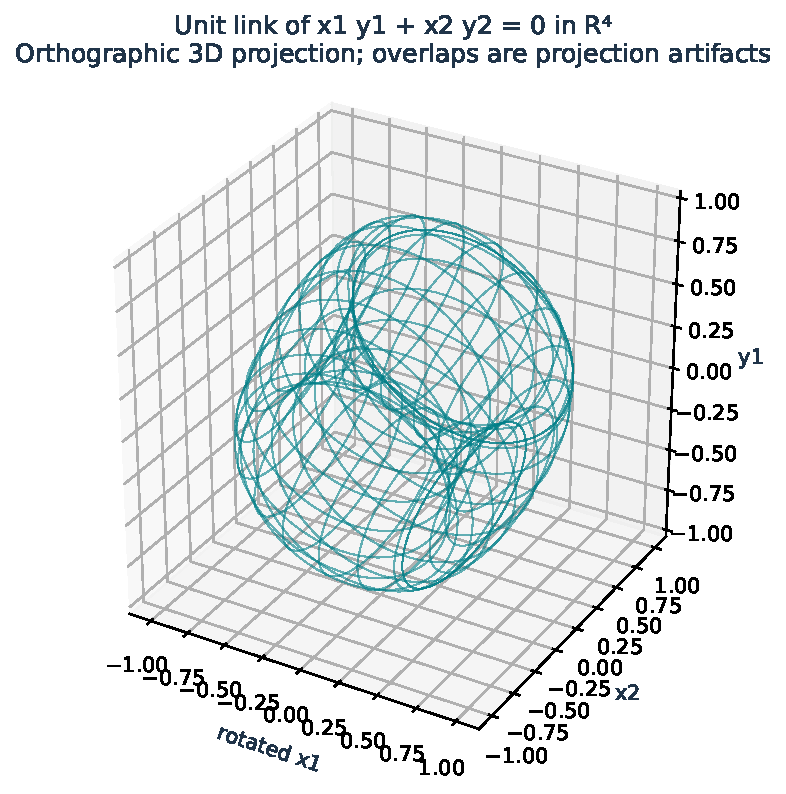
\includegraphics[width=.85\textwidth]{figures/cone_link.pdf}
\caption{A specified rotation in four-dimensional coordinate space followed
by orthographic projection into three dimensions. Apparent intersections
can be caused by projection. The mathematical link lies in $S^3\subset\R^4$;
it is not an embedded surface in ordinary three-dimensional space under
every projection.}
\end{figure}

The page exposes rotation and projection controls and reports the defining
equation's residual. Rank strata are derived from whether $A$ and $B$ vanish,
rather than inferred from the appearance of the projected image. The origin
is handled separately from the link. The tangent calculation is also
separate: a direction satisfying the linearized equation may retain a
quadratic obstruction, as proved and partially formalized in the companion.

\section{Index, kernel and gap are separate readouts}

For
\[
 A_\eps=(\eps,0)^T,\qquad B=(0,1),
\]
the middle Laplacian is $\diag(\eps^2,1)$. For $\eps\ne0$ the complex is exact
in the middle and its least eigenvalue is positive. As $\eps\to0$ the lowest
eigenvalue approaches zero. At $\eps=0$ the kernel dimension changes. The
Euler characteristic of the underlying three-term complex remains
$1-2+1=0$. At the endpoint, the smallest \emph{positive} eigenvalue is 1,
whereas the smallest eigenvalue is 0; these are different readouts and the
page distinguishes them.

\begin{figure}[htbp]
\centering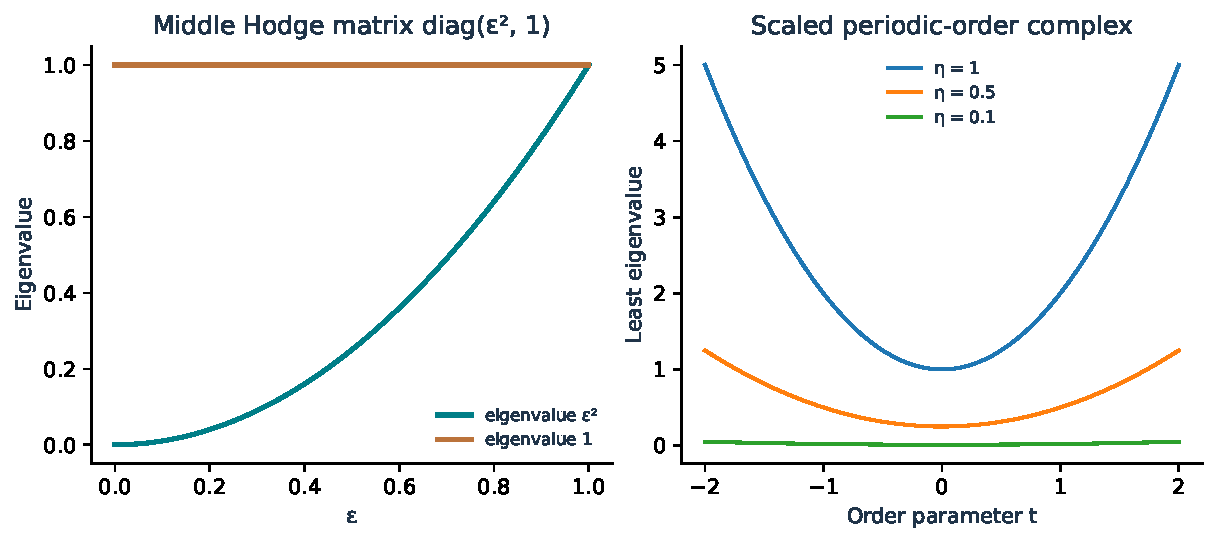
\includegraphics[width=\textwidth]{figures/hodge_gaps.pdf}
\caption{Left: a fixed Euler characteristic with changing kernel and lower
eigenvalue. Right: the exact periodic-order example has eigenvalue
$\eta^2(1+t^2)$ after rescaling both differentials. Algebraic exactness does
not determine a metric scale. These are finite matrices, not physical
Yang--Mills Hamiltonians.}
\end{figure}

The twisted flat-torus spectrum provides an infinite-dimensional counterpart
whose eigenvalues are still explicit. With $L_1=L_2=1$ and automorphy
parameters $(s,0)$ for $s\in[-1/2,1/2]$, its lowest scalar eigenvalue is
$4\pi^2s^2$. At the trivial character a zero mode appears. This plot belongs
to a free rank-one flat connection, and it must not be read as an interacting
nonabelian quantum mass-gap computation.

\begin{figure}[htbp]
\centering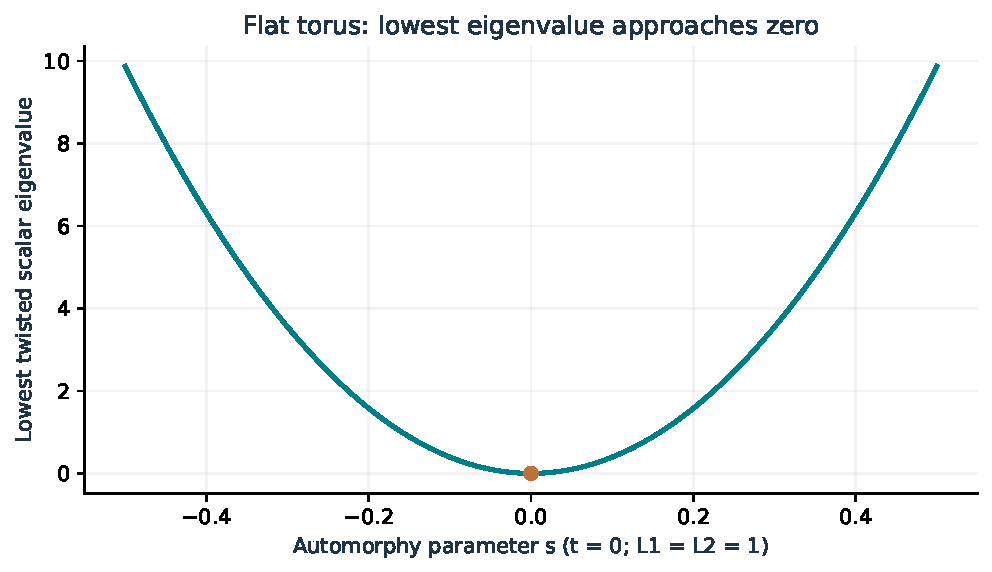
\includegraphics[width=.85\textwidth]{figures/twisted_gap.pdf}
\caption{An exact slice of the flat-torus spectral family. The horizontal
coordinate is an automorphy parameter modulo one; it is not time, energy,
or a lattice-spacing cutoff.}
\end{figure}

\section{The torus and plaquette displays}

The elliptic-torus laboratory starts with $\C/(\Z+\tau\Z)$, where
$\operatorname{Im}\tau>0$. A lattice Gram matrix records the flat metric of
the fundamental parallelogram. The familiar doughnut in three-dimensional
space is a topological visualization of the quotient, not an isometric
embedding of that flat metric. Changing $\tau$ changes the complex structure
and the displayed lattice data; an attractive three-dimensional surface
cannot substitute for those coordinates.

The optional gauge laboratory uses a single $U(1)$ plaquette. If edge
variables are $U_i$ and vertex transformations are $g_i$, then
\[
 U_i\longmapsto g_iU_ig_{i+1}^{-1}
\]
preserves the oriented product around the plaquette, since consecutive
factors cancel. For a nonabelian group the product is conjugated at the
base vertex and its trace is invariant. The browser displays the abelian
identity and a numerical residual. It does not generate a Yang--Mills
ensemble, take a continuum limit, or estimate a physical mass.

\section{Reproduction and interpretation}

The README gives commands for regenerating the JSON evidence and five
publication figures. Browser controls use native keyboard-accessible inputs;
the camera also supports keyboard rotation. Motion is user-controlled and
the reduced-motion preference is respected. Equations, parameter labels and
numeric summaries remain available alongside the canvas. The static
application uses relative links, so the same files can be served from a
local checkout or a project-hosting subdirectory.

Reproduction should begin with the small exact tests. If they fail, the
display should not be trusted. If they pass, that establishes consistency
for the tested examples, not every theorem in the paper. The next appendix
describes the different and stronger guarantee supplied by the selected
Lean declarations, together with the exact limits of that guarantee.

\section{Exact algebraic companion checks}
The gentle-invariant verification script checks all \(3^{10}=59{,}049\) ten-coordinate vectors with entries in \(\{0,1,2\}\), finds the 257 satisfying the four matching equations, and decomposes every one using the constructive proof. It also checks 100 larger constructed examples, the two corrected exponent relations, and 135 exact block determinants for the Kronecker pencil. Direct pair arithmetic in \(\F_{17}[u]/(u^2-3)\) counts 323 points on the companion elliptic curve, agreeing with the independently derived zeta recurrence. These results are recorded in \texttt{extension/verification/invariants.json}.

The interactive algebra companion has separate exact checks: 6,561 small Plucker matrices; all fifteen tableaux of shape \((3,2)\) on three letters; 2,478 admissible gentle rank cases, tested by independent elimination in characteristics two and seven; and 6,561 matching-generator monomials with 4,529 distinct exponent vectors. These finite tests verify implementations of the proved formulas; they are not substitutes for the unbounded proofs in the algebraic chapters.

The quantum companion and its GPU results are described in the quantum-surface chapter. The browser worker was also exercised through its actual controls: the 42-gate encoder produced support on 256 basis states with norm and all stabilizers equal to one to the displayed precision; an X error on edge zero flipped exactly the two adjacent face checks; and a live gradient update reduced the displayed loss with all sixteen predictions computed. Browser layout checks included a 375-pixel content viewport without page-level horizontal overflow.
